\documentclass{ximera}  
\title{Flowcharts with Operators}  
\begin{document}  
\begin{abstract}  
We introduce some mathematical notation to help us create algorithms to solve mathematical problems. 
\end{abstract}  
\maketitle

\section{Operators}
Many of the problems we will encounter in this course will require that we perform some iterative process or compute some quantity. For example:

\begin{enumerate}
	\item Compute $1+2+3+\cdots+16$.
	\item Count the number of divisors of $100$.
	\item Determine the value of your account after 10 years if you invest \$1000 into a savings account that offers a $4$\% interest rate compounded monthly.
	\item Sort the list of numbers 1, 5, 6, 2, 3, 8, 4 in ascending order.
\end{enumerate}

When creating algorithms to solve these types of problems, we will often need to compare quantities or keep track of (and update) certain values. To help us with this we introduce some important notation and conventions.

\begin{itemize}
	\item Assignment ($:=$) - This operator assigns the value of whatever is on the right to whatever is on the left. For example, $x:=2$ assigns the value $2$ to the variable $x$. Note that $x:=y$ and $y:=x$ are not the same. Also, a statement like $x:=x+1$ increments the value of $x$ by 1.
	\item Comparison ($=,<,>,<=,>=,!=$) - These operators are used for comparisons. They give back a truth value to help determine which route to take in a conditional operation/decision. For example, $x>0$ will be true if the value of $x$ is larger than $0$ and false otherwise.
	\item Arithmetic ($+,-,*,**,/,\%$) - These symbols simply perform the particular operations that we are used to. Note that $**$ represents exponentiation and $\%$ is modular division (it returns the remainder after long division). For example, $2**3 = 2^3 = 8$ and $7\%3 = 1$.
\end{itemize}

Here is an example of an algorithm that computes the sum $1+2+3+\cdots+n$ for any integer $n>0$.

\begin{center}
	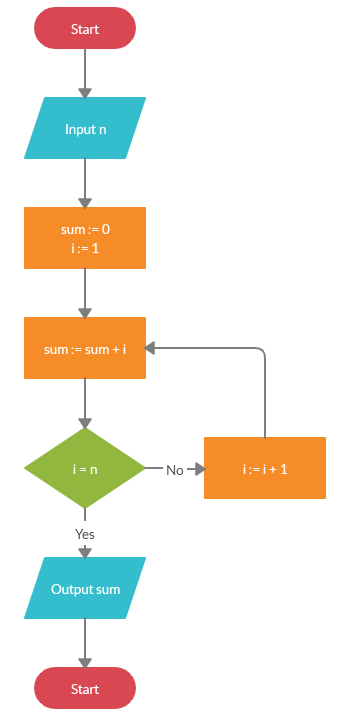
\includegraphics{gausssum2.png}
\end{center}

\section{Problems}

\begin{question}
	A divisor $m$ of $n$ is any integer $m$ such that there is no remainder when dividing $n$ by $m$. Create an algorithm that counts the number of divisors of $n$ for any integer $n>0$. 
	\begin{hint}
	You may need two decisions to solve this problem. Note that the second hint for this problem is the solution.
	\end{hint}

	\begin{hint}
	\begin{center}
		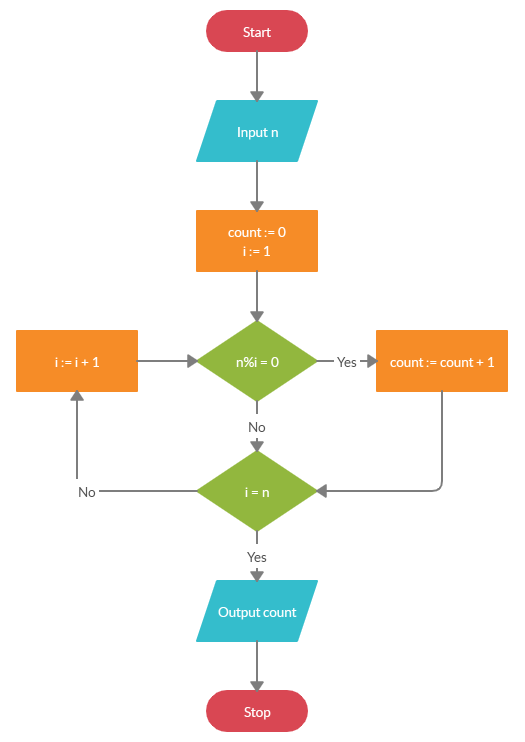
\includegraphics{divcount.png}
	\end{center}
	\end{hint}
\end{question}

\begin{question}
	Create an algorithm that determines if a positive integer is a prime number. Prime numbers are integers greater than 1 that have exactly two distinct divisors.
	\begin{hint}
		You should be able to modify the divisor count algorithm above.
	\end{hint}
\end{question}

\end{document}
